% !TEX root = ./main.tex
\documentclass[bigger,notes,aspectratio=169]{beamer}
\usetheme{metropolis}
\title{Bridging the gap between Typestates and Rust in production code}
\author{\textbf{José Duarte}\texorpdfstring{\\ António Ravara (Advisor)}{}}
\date{March 2021}
\institute{NOVA School of Science and Technology}

% \immediate\write18{if not exist tikz_external mkdir tikz_external}

\usepackage{tikz}
\usetikzlibrary{shapes,backgrounds,positioning}
\tikzset{
    invisible/.style={opacity=0,text opacity=0},
    normal/.style={opacity=1,text opacity=1},
    visible on/.style={alt=#1{}{invisible}},
    bold on/.style={alt=#1{font=\bfseries}{normal}},
    alt/.code args={<#1>#2#3}{%
      \alt<#1>{\pgfkeysalso{#2}}{\pgfkeysalso{#3}} % \pgfkeysalso doesn't change the path
    },
}
\usepackage{xcolor}

% \usepackage{pgfplots}
\usepackage{pgfpages}
\usepackage{hyperref}

% \usepgfplotslibrary{external}
% \tikzexternalize[
%     prefix={tikz_external/},
%     only named,
% ]

% \tikzset{
%     export as png/.style={
%         external/system call/.add={}{
%             ; convert -density #1 -transparent white "\image.pdf" "\image.png"
%         },
%     },
%     export as png/.default={200},
% }

\usepackage{amssymb}

\usepackage[newfloat]{minted}
\setminted{
    linenos,
    frame=single,
    style=lovelace,
    fontsize=\small,
}

\usepackage[main=american,portuguese]{babel}
\babeltags{pt=portuguese, enUS=american}

\setbeameroption{show notes on second screen}

\begin{document}

\begin{frame}[plain]
    \titlepage

    \note{
        \begin{pt}
            Bom dia Professor(es), sou o José Duarte, e o meu tema de tese é "Bridging the gap between typestates and Rust in production code".

            % O tema é orientado pelo Professor António Ravara.
        \end{pt}
    }
\end{frame}

\AtBeginSection[]
{
    \begin{frame}
        \frametitle{Outline}
        \tableofcontents[currentsection, hideothersubsections]
    \end{frame}
}

\section{Introduction}

\note{
    \begin{pt}
        A introdução segue a seguinte estrutura.
    \end{pt}
}

\subsection{Context}
\begin{frame}
    \frametitle{Context}
    Software plays a crucial role in our lives.
    \begin{itemize}
        \item From web browsers, to word processors and more!
    \end{itemize}

    As software becomes more important, bugs become more expensive.
    \begin{itemize}
        \item Losing work due to a bug in the save procedure is not nice.
        \item A bug in the firmware for a pacemaker may cost a life.
    \end{itemize}

    \note{
        \begin{pt}
            Dado o papel crescente do software nas nossas vidas,
            os bugs saem cada vez mais caro, tanto às empresas como aos utilizadores.

            Perder uma mensagem no Facebook não é grave, mas um dia de trabalho é pior.
            Imagine-se então um bug num pacemaker, pode causar a morte do utilizador!
        \end{pt}
    }
\end{frame}

\subsection{Problem}
\begin{frame}
    \frametitle{Problem --- in mainstream languages}
    \begin{figure}
        \centering
        \begin{tikzpicture}
            \def\fstcircle{(0, 0) circle (2.5)}
            \def\sndcircle{(0,-1.25) circle (1)}

            \fill[fill opacity=0.25, blue] \fstcircle;
            \fill[fill opacity=0.35, red] \sndcircle;

            \draw \fstcircle;
            \draw \sndcircle;

            \node at (0, 3) {Bugs};
            \node at (0, 1.25) {Preventable};
            \node at (0, -1.25) {\scriptsize Prevented};
        \end{tikzpicture}
        \caption{Diagram of preventable bugs and prevented bugs.}
    \end{figure}

    \note{
        \begin{pt}
            Podemos imaginar todos os tipos de bugs como um conjunto (não mostrado),
            onde se inserem dois subconjuntos.
            Os bugs que podemos prevenir e os que, de facto, conseguimos prevenir.

            Os que prevenimos são, por exemplo, type mismatch errors;
            os erros que não conseguimos produzir são, por exemplo, gestão de memória.
        \end{pt}
    }
\end{frame}

\begin{frame}
    \frametitle{Problem --- with Rust}
    \begin{figure}
        \centering
        \begin{tikzpicture}
            \def\fstcircle{(0,0) circle (2.5)}
            \def\sndcircle{(0,-.75) circle (1.5)}

            \fill[fill opacity=0.25, blue] \fstcircle;
            \fill[fill opacity=0.35, red] \sndcircle;

            \draw \fstcircle;
            \draw \sndcircle;

            \node at (0, 3) {Bugs};
            \node at (0, 1.25) {Preventable};
            \node at (0, -.75) {Prevented};
        \end{tikzpicture}
        \caption{Diagram of preventable bugs and prevented bugs when considering Rust's borrow checker.}
    \end{figure}

    \note{
        \begin{pt}
            Rust permite-nos alargar o conjunto de bugs que conseguimos prevenir,
            incluindo assim os bugs de memória e de concurrência.

            No entanto, continua a não conseguir cobrir todos os bugs.
        \end{pt}
    }
\end{frame}

\begin{frame}
    \frametitle{Problem --- Ideal}
    \begin{figure}
        \centering
        \begin{tikzpicture}
            \def\X{0}
            \def\fstX{-\X}
            \def\sndX{\X}
            \def\Y{0}
            \def\fstcircle{(\fstX,0) circle (2.5)}
            \def\sndcircle{(\sndX,0) circle (2.5)}

            \fill[fill opacity=0.25, blue] \fstcircle;
            \fill[fill opacity=0.35, red] \sndcircle;

            \draw \fstcircle;
            \draw \sndcircle;

            \node at (0, 3) {Bugs};
            \node at (0, 0) {Preventable \& Prevented};
        \end{tikzpicture}
        \caption{The ideal diagram of preventable bugs and prevented bugs, where all bugs are prevented.}
    \end{figure}
    \note{
        \begin{pt}
            O ideal seria uma sobreposição total, como na figura.
            Os typestates ajudam-nos a dar um passo nesta direção.

            Apesar da programação defensiva tentar maximizar os erros prevenidos,
            existe sempre o limite do erro humano.
        \end{pt}
    }
\end{frame}

% \subsection{Problem}
\begin{frame}[fragile]
    \frametitle{Problem} % ???
    Error happens at runtime, possibly crashing the program.
    \begin{listing}
        \centering
        \begin{minted}{Rust}
fn main() {
    let builder = XYBuilder::new();
    builder.setX(0.0);
    builder.build(); // runtime error: missing `y`
}
        \end{minted}
    \end{listing}
    Our tools should work for us, not make us work for them.

    \note{
        \begin{pt}
            Queremos diminuir os bugs.
            No entanto, os bugs que queremos endereçar são principalmente maus usos das APIs.

            Como na figura, o programa iria lançar um panico porque não inicializei o Y.

            Enquanto programadores, queremos que a máquina trabalhe por nós, não ao contrário.
            Minimizando assim o tempo de debug, e a complexidade associada ao trabalho.
        \end{pt}
    }
\end{frame}

\subsection{Objectives}

\begin{frame}
    \frametitle{What are typestates?}

    \begin{itemize}
        \item An approach to behavioral types.
        \item Allow the developer to cleanly and concisely express API constraints.
    \end{itemize}

    \emph{e.g. “Do not call \texttt{.next()} before \texttt{.hasNext()}.”}

    \note{
        \begin{pt}
            Typestates são uma abordagem a tipos comportamentais.
            Estes visam descrever o estado em runtime do programa através do sistema de tipos.

            Podem ser modelados como máquinas de estados e permitem ao programador expressar de forma clara e consisa restrições de uso de uma API.
        \end{pt}
    }
\end{frame}


\begin{frame}
    \frametitle{Objectives}
    A library which brings \emph{practical} typestates to Rust.
    \begin{itemize}
        \item Minimal learning overhead.
              % \item Zero-cost abstraction.
        \item Scalable to large projects.
    \end{itemize}


    \note{
        \begin{pt}
            Esta tese visa então providenciar typestates práticos na linguagem Rust.

            Os mesmos:
            \begin{itemize}
                \item Devem ser fáceis de aprender e usar.
                \item Devem escalar a projetos grandes.
            \end{itemize}
        \end{pt}
    }
\end{frame}

\section{State of the Art}
\note{
    \begin{pt}
        Devido a restrições de tempo vou cingir-me a implementações de tipos comportamentais para linguagens
        de alto nível em linha com a minha abordagem.
    \end{pt}
}
\subsection{Session Types}
\begin{frame}[fragile]
    \frametitle{Session Types --- StMungo}
    StMungo is a tool that converts Scribble protocols into a Mungo typestate specification and Java skeleton.

    \begin{minipage}{0.3\linewidth}
        \begin{figure}
            \centering
            \begin{tikzpicture}
                \node (scribble) at (0,  0) {Scribble};
                \node (java)     at (2.25,  1.25) {Java};
                \node (mungo)    at (2.25, -1.25) {Mungo};

                \draw[->, thick] (scribble) edge[out=0, in=180] (java);
                \draw[->, thick] (scribble) edge[out=0, in=180] (mungo);
                \draw[->, thick, dashed] (mungo) -- node[right, font=\scriptsize\itshape] {Checks} (java);
            \end{tikzpicture}
        \end{figure}
    \end{minipage}\hfill%
    \begin{minipage}{0.33\linewidth}
        \begin{listing}
            \centering
            \begin{minted}[fontsize=\tiny, linenos=false]{text}
module example;

type <xsd> "..."
    from "..." as Hello;

global protocol P(role A, role B) {
    connect(Hello) from A to B;
}
            \end{minted}
        \end{listing}
    \end{minipage}\hfill%
    \begin{minipage}{0.25\linewidth}
        \begin{listing}
            \centering
            \begin{minted}[fontsize=\tiny, linenos=false]{java}
typestate Protocol {
    Init  =
        { /* ... */ }
    Close =
        { /* ... */ }
}
            \end{minted}
        \end{listing}
    \end{minipage}
    \note{
        \begin{pt}
            O StMungo (ou Scribble to Mungo) é uma ferramenta que converte protocolos de Scribble para especificações de typestates em Mungo e esqueletos de API em Java.
            A implementação Java é depois verificada pelo Mungo.

            O Scribble permite ainda a conversão de multiparty session types para binary session types.
        \end{pt}
    }
\end{frame}

\begin{frame}
    \frametitle{Session Types --- Session Types \& Rust}
    % The first work with session types and Rust.

    % Exploits the type system to provide binary session types checked at compile-time.

    % The library makes use of \texttt{unsafe} features.

    \begin{table}
        \centering
        \begin{tabular}{l|l|l|l}
                                & Kind       & Compile-Time & Ext. Tool  \\
            \hline
            Jespersen et al.    & Binary     & \checkmark   &            \\
            \hline
            Lagaillardie et al. & Multiparty & \checkmark   & \checkmark
        \end{tabular}
    \end{table}

    \note{
        \begin{pt}
            (Tanto quanto sei) O trabalho de Jespersen et al. foi o primeiro a introduzir session types em Rust,
            entre esse e o seu principal sucessor as diferenças residem no suporte de multiparty session types e o uso ferramentas externas.
            Ambos válidos para o seu sucessor Lagaillardie.

            Os trabalhos apresentados providenciam tipos apenas para canais.
        \end{pt}
    }
\end{frame}

\subsection{Typestates}

\begin{frame}
    \frametitle{Typestates --- Plaid}
    Plaid is a \emph{typestate-oriented} language.

    It also supports aliasing control through keyword usage:
    \begin{table}
        \centering
        \begin{tabular}{l|l|l}
                               & Aliasing   & Mutation   \\
            \hline
            \texttt{unique}    &            & \checkmark \\
            \hline
            \texttt{immutable} & \checkmark &            \\
            \hline
            \texttt{shared}    & \checkmark & \checkmark
        \end{tabular}
    \end{table}

    \note{
        \begin{pt}
            O Plaid é uma linguagem orientada aos typestates, fazendo uso dos mesmos como cidadãos de primeira classe.

            A outra caracteristica mais relevante da linguagem é o seu controlo de aliasing,
            efetuado através de palavras-chave, como descrito na tabela.
        \end{pt}
    }
\end{frame}

\begin{frame}[fragile]
    \frametitle{Typestates --- Fugue}
    \begin{listing}
        \centering
        \begin{minted}{csharp}
[WithProtocol("open", "closed")]
class OuterSocket {
    [InState("connected",
        WhenEnclosingState="open"),
     NotAliased(WhenEnclosingState="open")]
    [Unavailable(WhenEnclosingState="closed")]
    private Socket innerSocket;
}
        \end{minted}
    \end{listing}

    \note{
        \begin{pt}
            Seguindo então para os typestates, começo com o Fugue.
            Um projeto vindo da Microsoft, onde o meu trabalho se inspira.

            O Fugue permite a descrição de estados e transições através de anotações.

            Permite ainda a ligação entre sub-estados para garantir o bom uso das APIs.
        \end{pt}
    }
\end{frame}

\begin{frame}[fragile]
    \frametitle{Typestates --- Mungo}
    \begin{figure}
        \centering
        \begin{tikzpicture}
            \tikzstyle{state} = [circle, thick, minimum size=0.6cm, draw=black!70, font=\scriptsize\ttfamily]
            \tikzstyle{transition} = [->, thick, draw=black!70]
            \node[state, label=above:{\scriptsize\ttfamily Init}] (init) at (0, 0) {};
            \node[state, label=above:{\scriptsize\ttfamily Open}] (open) at (2, 0) {};
            \node[state, label=above:{\scriptsize\ttfamily Close}] (close) at (4, 0) {};
            \node[state, label=above:{\scriptsize\ttfamily end}] (end) at (6, 0) {};
            \node[state, minimum size= 0.45cm] (inner-end) at (6, 0) {};
            \draw[transition] (init) -- node[above, font=\tiny\ttfamily] {open:OK} (open);
            \draw[transition] (init) -- (0, -0.85) -- node[below, font=\tiny\ttfamily] {open:ERROR} (6, -0.85) -- (end);
            \draw[transition] (open) -- node[above, font=\tiny\ttfamily] {read:EOF} (close);
            \draw[transition] (open) edge[loop below] node[above right, font=\tiny\ttfamily] {read:OK} (open);
            \draw[transition] (close) -- node[above, font=\tiny\ttfamily] {close} (end);
        \end{tikzpicture}
    \end{figure}

    \begin{listing}
        \centering
        \begin{minted}[fontsize=\footnotesize]{java}
@Typestate("SocketProtocol")
class Socket { /* ... */ }
        \end{minted}
    \end{listing}
    \begin{listing}
        \centering
        \begin{minted}[fontsize=\footnotesize]{java}
typestate Socket {
    Init  = { Status open(): <OK: Open, ERROR: end> }
    Open  = { Read read(): <OK: Open; EOF: Close> }
    Close = { void close(): end }
}
        \end{minted}
    \end{listing}

    \note{
        \begin{pt}
            Por fim temos o Mungo, já falado antes mas não apresentado formalmente.
            O Mungo é um sistema de tipos / um verificador de typestates.

            O seu uso em Java consiste no processamento de uma anotação que liga a descrição do typestate de uma classe,
            após o processamento da anotação, o Mungo verifica todos os usos da classe validando os mesmos contra a especificação.
        \end{pt}
    }
\end{frame}

\section{Case Study}

\note{
    \begin{pt}
        Apresento agora o caso de estudo de acordo com a seguinte estrutura.
    \end{pt}
}

\begin{frame}[fragile]
    \frametitle{Problem} % ???
    \begin{listing}
        \centering
        \begin{minted}{Rust}
fn main() {
    let builder = XYBuilder::new();
    builder.setX(0.0);
    builder.build(); // runtime error: missing `y`
}
        \end{minted}
    \end{listing}
    \note{
        \begin{pt}
            Para relembrar, o problema é o compilador não avisar que aquela chamada está fora de ordem.
        \end{pt}
    }
\end{frame}

\subsection{Solution}
\begin{frame}[fragile]
    \frametitle{Solution}
    Ideally, we want to catch the error at compile-time.
    \begin{listing}
        \centering
        \begin{minted}{Rust}
fn main() {
    let builder = XYBuilder::new();
    builder.setX(0.0);
    builder.build();
         // ^^^^^
         // | error: you cannot build without setting `y`
}
        \end{minted}
    \end{listing}

    \emph{How?}
    \only<2>{Declare the protocol.}

    \note{
        \begin{pt}
            Nós queremos que o compilador nos diga "hey, não podes chamar este método nesta altura".
            Como é que o podemos fazer?
        \end{pt}
    }
\end{frame}

\subsection{Approach}
\begin{frame}
    \frametitle{Approach --- Overview}

    \emph{\textbf{We can exploit the Rust typesystem to emulate typestates.}}

    \begin{overprint}
        \onslide<2->{However this approach requires boilerplate.}

        \onslide<3->{Use macros! Part of the language, requiring no new experience.}
        \begin{itemize}
            \item<4-> Rewrite the annotated code, generating boilerplate for the user.
            \item<5-> Throw errors during compile-time.
        \end{itemize}
    \end{overprint}

    \note{
        \begin{pt}
            Usando o sistema de tipos de Rust, podemos emular typestates.
            No entanto, esta abordagem requer muito boilerplate.

            Esta abordagem não requer um esforço especial por parte do utilizador, visto que os macros são um elemento comum da linguagem.

            Usando macros, podemos gerar o código por nós.
            Podemos ainda validar o código contra outras propriedades e lançar erros durante a compilação.
        \end{pt}
    }
\end{frame}

\begin{frame}<1-5>[fragile]
    \frametitle{Approach --- Going deeper}
    \setmintedinline[rust]{fontsize=\tiny}
    % \begin{overprint}
    \begin{figure}
        \centering
        \begin{tikzpicture}
            \tikzstyle{Code} = [align=left]
            \tikzstyle{Text} = [align=center, font=\small, fill=none]
            \tikzstyle{Conn} = [above, align=center, font=\itshape\scriptsize, fill=none]
            \tikzstyle{Node} = [circle, draw=blue!70, fill=blue!30, minimum size=0.1cm]
            \tikzstyle{FSMS} = [circle, draw=green!70, fill=green!30, minimum size=0.1cm]
            \tikzstyle{FSME} = [circle, draw=red!70, fill=red!30, minimum size=0.1cm]
            \node[Text, bold on=<2>] (ts-spec) at (0, 4) {Typestate\\Specification};
            \node[Text, bold on=<3>] (ts-ast)  at (3, 4) {AST};
            \node[Text, bold on=<4>] (ts-fsm)  at (6, 4) {State\\Machine};
            \node[Text, bold on=<5>] (ts-code) at (9, 4) {Rust\\Code};

            \draw[->] (ts-spec) -- node[Conn] {Parse} (ts-ast);
            \draw[->] (ts-ast)  -- node[Conn] {Convert} (ts-fsm);
            \draw[->] (ts-fsm)  -- node[Conn] {Check: Ok} (ts-code);
            \draw[->] (ts-fsm)  edge[in=35, out=145] node[Conn] {Check: Error} (ts-spec);

            \begin{scope}[shift={(0, 2)}]
                \node[Code] (ts-spec-code) at (0,0) {\mintinline{rust}{#[typestate]}\\\mintinline{rust}{// ...}};
            \end{scope}

            \begin{scope}[shift={(3, 1)}]
                \node[Node] (n0) at (0, 2) {};
                \node[Node] (n1) at (-0.5, 1) {};
                \node[Node] (n2) at (0.5, 1) {};
                \node[Node] (n3) at (0, 0) {};
                \node[Node] (n4) at (1, 0) {};
                \draw[-] (n0) -- (n1);
                \draw[-] (n0) -- (n2);
                \draw[-] (n2) -- (n3);
                \draw[-] (n2) -- (n4);
            \end{scope}

            \begin{scope}[shift={(6, 1)}]
                \node[FSMS] (n0) at (0, 2) {};
                \node[Node] (n1) at (-0.5, 1) {};
                \node[Node] (n2) at (0.5, 1) {};
                \node[FSME] (n3) at (0, 0) {};
                \draw[->] (n0) -- (n1);
                \draw[->] (n0) -- (n2);
                \draw[->] (n1) -- (n2);
                \draw[->] (n2) -- (n3);
            \end{scope}

            \begin{scope}[shift={(9, 2)}]
                \node[Code] (ts-spec-code) at (0,0) {
                    \mintinline{rust}{struct S { ... }}\\
                    \mintinline{rust}{trait SOps { ... }}\\
                    \mintinline{rust}{// ...}
                };
            \end{scope}

            \draw[dashed] (1.5, 1) -- (1.5, 3);
            \draw[dashed] (4.5, 1) -- (4.5, 3);
            \draw[dashed] (7.5, 1) -- (7.5, 3);
        \end{tikzpicture}
    \end{figure}
    % \end{overprint}

    \note{
        \begin{pt}
            Aprofundando, para fazer com que tal aconteça a arquitetura do macro será como na figura.
            A especificação é código Rust normal, recorrendo a macros.

            Daí, o sistema de macros extrai a AST,
            a qual precisamos apenas de processar para extrair uma máquina de estados e gerar o código final.

            A máquina de estados extraída é verificada para uma série de propriedades e se tudo estiver OK, podemos gerar o código final.
            Caso contrário, podemos lançar um erro de compilação.
        \end{pt}
    }
\end{frame}

\subsection{Workflow}
\begin{frame}[fragile]
    \frametitle{Workflow --- Design the state machine}
    Consider a traffic light as a state machine.
    \begin{figure}
        \centering
        % \tikzset{export as png}
        % \tikzsetnextfilename{traffic_light_fsm}
        \begin{tikzpicture}
            \tikzstyle{state} = [circle, thick, minimum size=0.75cm]
            \tikzstyle{transition} = [->, very thick, draw=black!70]
            \node[circle, thick, dashed, minimum size=0.75cm, draw=black!70] (off) at (0, 0) {};
            \node[circle, thick, minimum size=0.6cm, draw=black!70, fill opacity=0] at (0, 0) {};
            \node[state, draw=red!70, fill=red!30] (r) at (3, 0) {};
            \node[state, draw=yellow, fill=yellow!50] (y) at (6, 0) {};
            \node[state, draw=green!70, fill=green!30] (g) at (10, 0) {};
            \draw[transition] (g) -- node[above, font=\small\ttfamily] {to\_yellow} (y);
            \draw[transition] (y) -- node[above, font=\small\ttfamily] {to\_red} (r);
            \draw[transition] (r) edge[in=-150, out=-30] node[below, font=\small\ttfamily] {to\_green} (g);
            \draw[transition] (off) edge[in=-135, out=-45] node[below, font=\small\ttfamily] {turn\_on} (r);
            \draw[transition] (r) -- node[above, font=\small\ttfamily] {turn\_off} (off);
            \draw[transition] (-1, 0) -- (off);
        \end{tikzpicture}
    \end{figure}

    \note{
        \begin{pt}
            Consideremos um semáforo.
            Ele percorre um ciclo, verde, amarelo, vermelho e o mesmo pode ser ligado e desligado.

            Vamos então modelá-lo com a biblioteca.
        \end{pt}
    }
\end{frame}

\begin{frame}[fragile]
    \frametitle{Workflow --- Declaring state in Rust}
    Using the DSL we first declare the module, main automata and the states:
    \begin{listing}
        \centering
        \begin{minted}{rust}
#[typestate] mod traffic_light {
    #[automata] struct TrafficLight;
    #[state] struct Green;
    #[state] struct Yellow;
    #[state] struct Red;
    // ...
        \end{minted}
    \end{listing}
    We still need transitions!

    \note{
        \begin{pt}
            Começamos por declarar o autómato e os estados do mesmo.
        \end{pt}
    }
\end{frame}

\begin{frame}[fragile]
    \frametitle{Workflow --- Declaring transitions in Rust}
    All transition functions take ownership of the current state and return the new state.
    \begin{listing}
        \centering
        \begin{minted}{rust}
    // code from the previous slide ...
    fn to_yellow(self: Green) -> Yellow;
    fn to_red(self: Yellow) -> Red;
    fn to_green(self: Red) -> Green;
    // ...
        \end{minted}
    \end{listing}

    \note{
        \begin{pt}
            De seguida, as transições entre estados.

            Note-se o consumo do estado atual e o retorno do novo estado.
        \end{pt}
    }
\end{frame}

\begin{frame}[fragile]
    \frametitle{Workflow --- Declaring \emph{start} states in Rust}
    Functions that do not use \texttt{self} and \emph{return} a valid state are inferred as the \emph{start} state.

    \begin{listing}
        \centering
        \begin{minted}{rust}
    // code from the previous slides ...
    fn turn_on() -> Red;
        \end{minted}
    \end{listing}

    \note{
        \begin{pt}
            Por fim, o estado inicial e final, que neste caso é o mesmo.

            Funções que não consomem o estado atual e retornam um estado são consideradas declarações de estados iniciais.

            Funções que consomem o estado atual e não retornam um estado são consideradas declarações de estados finais.
        \end{pt}
    }
\end{frame}

\begin{frame}[fragile]
    \frametitle{Workflow --- Declaring \emph{end} states in Rust}

    Functions that take \texttt{self} and do \emph{not return }a valid state are inferred as the \emph{end} state.
    \begin{listing}
        \centering
        \begin{minted}{rust}
    fn turn_off(self: Red);
}
        \end{minted}
    \end{listing}
    Our traffic light is ready!

    \note{
        \begin{pt}
            Por fim, o estado inicial e final, que neste caso é o mesmo.

            Funções que não consomem o estado atual e retornam um estado são consideradas declarações de estados iniciais.

            Funções que consomem o estado atual e não retornam um estado são consideradas declarações de estados finais.
        \end{pt}
    }
\end{frame}

\begin{frame}[fragile]
    \frametitle{Workflow --- The other features}
    For maintenance purposes, consider that our traffic light is now required to count every \texttt{GYR} cycle. % Green->Yellow->Red

    The \texttt{TrafficLight} structure is now declared as follows:
    \begin{listing}
        \centering
        \begin{minted}{rust}
#[automata] struct TrafficLight { cycles: u64 }
        \end{minted}
    \end{listing}

    \note{
        \begin{pt}
            Existem ainda mais alguns detalhes a apresentar.

            Imaginemos que queremos saber o número de ciclos atravessados pelo semáforo, para questões de manutenção.

            Adicionamos então um campo novo ao autómato, tornando-o disponível em todos os estados.
        \end{pt}
    }
\end{frame}

\begin{frame}[fragile]
    \frametitle{Workflow --- The other features}
    How can we check if the light requires maintenance?

    We add a \texttt{pure} function:
    \begin{listing}
        \centering
        \begin{minted}{rust}
fn requires_maintenance(self: &TrafficLight) -> bool;
        \end{minted}
    \end{listing}
    This function is not able to perform mutations due to the immutable reference (\texttt{\&}).

    \note{
        \begin{pt}
            Para confirmar se o semáforo precisa de manutenção criamos um predicado.
            Neste caso, a função só tem acesso imutável a uma referência de qualquer estado.
            Sendo assim uma função pura.
        \end{pt}
    }
\end{frame}

\begin{frame}[fragile]
    \frametitle{Workflow --- The other features}
    After maintenance, how can we reset the counter?

    We add an \texttt{impure} function:
    \begin{listing}
        \centering
        \begin{minted}{rust}
fn reset_counter(self: &mut TrafficLight);
        \end{minted}
    \end{listing}
    The function is able to perform mutations over fields, due to usage of a mutable reference (\texttt{\&mut}),
    \emph{but it is unable to transition between states}.

    \note{
        \begin{pt}
            Após a manutenção, é prático poder dar reset ao semáforo.
            Para tal usamos uma função impura, capaz de mutar o estado atual, mas não de fazer transições.
        \end{pt}
    }
\end{frame}

\begin{frame}[fragile]
    \frametitle{Workflow --- The new state machine}
    With the new methods the state machine now looks like:
    \begin{figure}
        \centering
        \begin{tikzpicture}
            \tikzstyle{state} = [circle, thick, minimum size=0.75cm]
            \tikzstyle{transition} = [->, very thick, draw=black!70]
            \node[circle, thick, dashed, minimum size=0.75cm, draw=black!70] (off) at (0, 0) {};
            \node[circle, thick, minimum size=0.6cm, draw=black!70, fill opacity=0] at (0, 0) {};
            \node[state, draw=red!70, fill=red!30] (r) at (3, 0) {};
            \node[state, draw=yellow, fill=yellow!50] (y) at (6, 0) {};
            \node[state, draw=green!70, fill=green!30] (g) at (10, 0) {};
            \draw[transition] (g) -- node[above, font=\small\ttfamily] {to\_yellow} (y);
            \draw[transition] (y) -- node[above, font=\small\ttfamily] {to\_red} (r);
            \draw[transition] (r) edge[in=-150, out=-30] node[below, font=\small\ttfamily] {to\_green} (g);
            \draw[transition] (off) edge[in=-135, out=-45] node[below, font=\small\ttfamily] {turn\_on} (r);
            \draw[transition] (r) -- node[above, font=\small\ttfamily] {turn\_off} (off);
            \draw[transition] (-1, 0) -- (off);

            \draw[transition] (r) edge[loop above] node[above, font=\small\ttfamily]{*} (r);
            \draw[transition] (y) edge[loop above] node[above, font=\small\ttfamily]{*} (y);
            \draw[transition] (g) edge[loop above] node[above, font=\small\ttfamily]{*} (g);
        \end{tikzpicture}
    \end{figure}
    \begin{listing}
        \begin{minted}[linenos=false, frame=none]{text}
*: requires_maintenance
   reset_counter
        \end{minted}
    \end{listing}
    \note{
        \begin{pt}
            Após a adição das novas funcções, ficamos com a seguinte máquina de estados.
        \end{pt}
    }
\end{frame}

\begin{frame}[fragile]
    \frametitle{Workflow --- Final steps}
    After the code is checked and expanded, all that is left is for the user to implement the state transitions.
    \begin{listing}
        \centering
        \begin{minted}{rust}
impl GreenState for TrafficLight<Green> {
    fn to_yellow(self) -> TrafficLight<Yellow> {
        /* ... */
    }
}
        \end{minted}
    \end{listing}

    \note{
        \begin{pt}
            É possível adicionar a implementação diretamente às declarações das funções,
            no entanto, tal poderia tornar o código díficil de ler devido às transformações necessárias ao código.
        \end{pt}
    }
\end{frame}

\begin{frame}[fragile]
    \frametitle{Workflow --- Usage}
    The final user API would look like the following:
    \begin{listing}
        \centering
        \begin{minted}[highlightlines=1,highlightcolor=blue!10]{rust}
let tl = TrafficLight<Red>::turn_on();
let green = tl.to_green();
if green.requires_maintenance() {
    // ...
    green.reset();
}
green.to_red(); // compile-time error
        \end{minted}
    \end{listing}

    \note{
        \begin{pt}
            A API apresentada ao utilizador final seria a seguinte.

            O erro é apanhado pelo compilador, devido a um "type mismatch".
        \end{pt}
    }
\end{frame}

\begin{frame}[fragile]
    \frametitle{Workflow --- Usage}
    The final user API would look like the following:
    \begin{listing}
        \centering
        \begin{minted}[highlightlines=2,highlightcolor=blue!10]{rust}
let tl = TrafficLight<Red>::turn_on();
let green = tl.to_green();
if green.requires_maintenance() {
    // ...
    green.reset();
}
green.to_red(); // compile-time error
        \end{minted}
    \end{listing}

    \note{
        \begin{pt}
            A API apresentada ao utilizador final seria a seguinte.

            O erro é apanhado pelo compilador, devido a um "type mismatch".
        \end{pt}
    }
\end{frame}

\begin{frame}[fragile]
    \frametitle{Workflow --- Usage}
    The final user API would look like the following:
    \begin{listing}
        \centering
        \begin{minted}[highlightlines=3-6,highlightcolor=blue!10]{rust}
let tl = TrafficLight<Red>::turn_on();
let green = tl.to_green();
if green.requires_maintenance() {
    // ...
    green.reset();
}
green.to_red(); // compile-time error
        \end{minted}
    \end{listing}

    \note{
        \begin{pt}
            A API apresentada ao utilizador final seria a seguinte.

            O erro é apanhado pelo compilador, devido a um "type mismatch".
        \end{pt}
    }
\end{frame}

\begin{frame}[fragile]
    \frametitle{Workflow --- Usage}
    The final user API would look like the following:
    \begin{listing}
        \centering
        \begin{minted}[highlightlines=7,highlightcolor=red!10]{rust}
let tl = TrafficLight<Red>::turn_on();
let green = tl.to_green();
if green.requires_maintenance() {
    // ...
    green.reset();
}
green.to_red(); // compile-time error
        \end{minted}
    \end{listing}

    \note{
        \begin{pt}
            A API apresentada ao utilizador final seria a seguinte.

            O erro é apanhado pelo compilador, devido a um "type mismatch".
        \end{pt}
    }
\end{frame}

\section{Plan}

\begin{frame}
    \frametitle{Plan Overview}

    \begin{figure}[h]
        \centering
        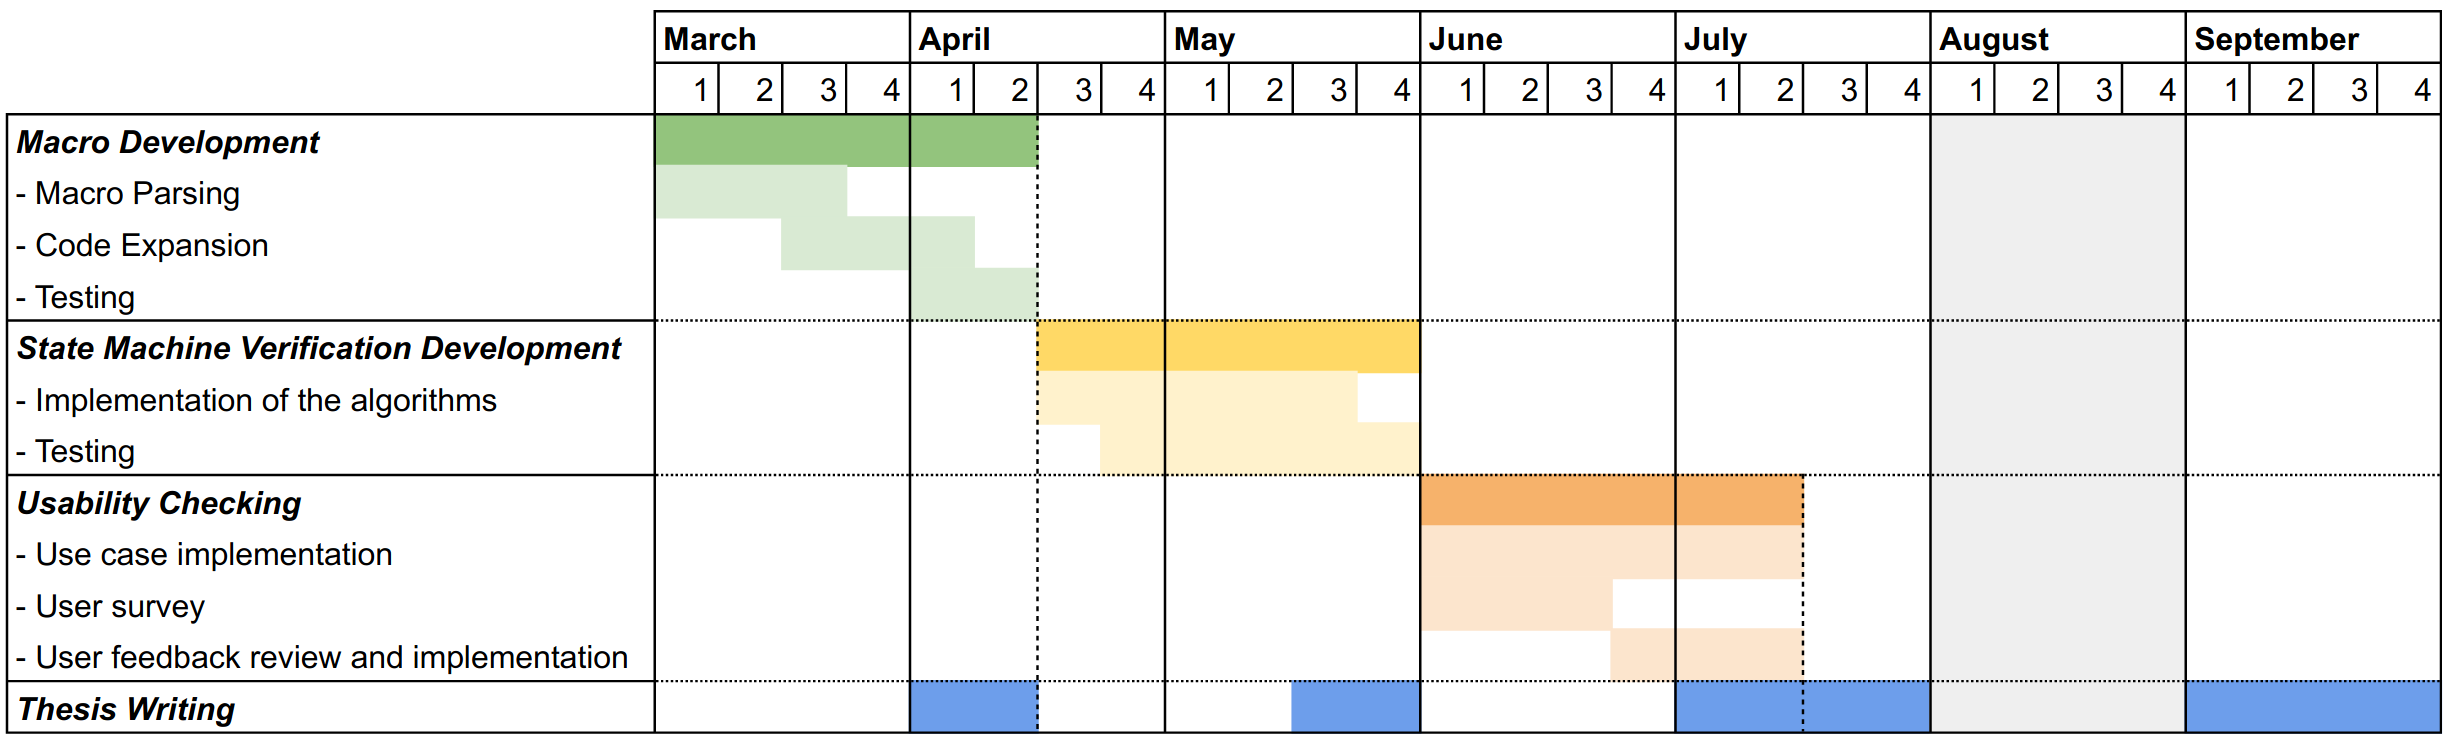
\includegraphics[width=\linewidth]{planning.png}
        \caption{Work plan Gantt chart}
    \end{figure}

    \note{
        \begin{pt}
            Por fim, apresento o plano de trabalho.

            (Apresentar e explicar a tabela.)
        \end{pt}
    }
\end{frame}

\end{document}